\chapter{DESAIN DAN IMPLEMENTASI}
\label{chap:desainimplementasi}

% Ubah bagian-bagian berikut dengan isi dari desain dan implementasi
Bab ini akan menjelaskan mengenai sistem perencanaan gerakan mobil otonom, mulai dari konfigurasi sensor pada Simulator mobil otonom, perancangan informasi dan parameter lingkungan berkendara pada Simulator mobil otonom, perancangan sistem berkendara mobil otonom, hingga perancangan arsitektur algoritma DQN yang digunakan dalam Tugas Akhir ini.


\section{Deskripsi Sistem}
\label{sec:deskripsisistem}

Sistem pada tugas akhir ini merupakan implementasi dari salah satu disiplin ilmu \textit{Deep Reinforcement Learning} yang berfungsi untuk menciptakan algoritma yang dapat melakukan manuver kendaraan otonom untuk bergerak melewati bundaran atau \textit{u-turn}. Blok diagram metodologi sistem yang digunakan pada penelitian ini dapat dilihat pada Gambar \ref{fig:blockdiagram}.

\section{Persiapan Lingkungan Simulasi}
\label{sec:simulasi}
Menggunakan simulator CARLA, digunakan map Town03 CARLA, yang memiliki bundaran dan u-turn untuk memfasilitasi pengerjaan tugas akhir. Terdapat dua jenis bundaran yang digunakan pada tugas akhir ini.

\subsection{Bundaran Simpang Empat}
Digunakan bundaran berjumlah simpang empat seperti pada Gambar  \ref{fig:bundaran_town03}. Pada lingkungan ini, agent akan \textit{spawn }dari empat titik \textit{spawn} di sekitar bundaran.
\begin{figure}[H] 
	\centering
	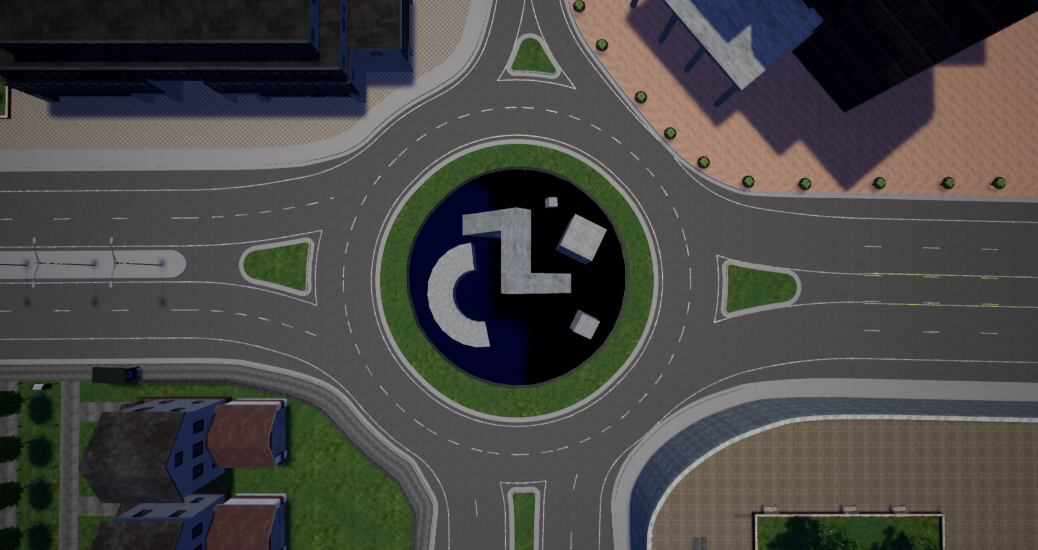
\includegraphics[width=.7\linewidth]{images/bundaran}
	\caption{Bundaran Simpang Empat}
	\label{fig:bundaran_town03}
\end{figure}

\subsection{Bundaran Tanpa Simpang}
Digunakan bundaran tanpa simpang seperti pada Gambar  \ref{fig:bundaran_tanpa_simpang}. Pada lingkungan ini, agent akan \textit{spawn }dari sebuah titik \textit{spawn} awal bundaran.
\begin{figure}[H] 
	\centering
	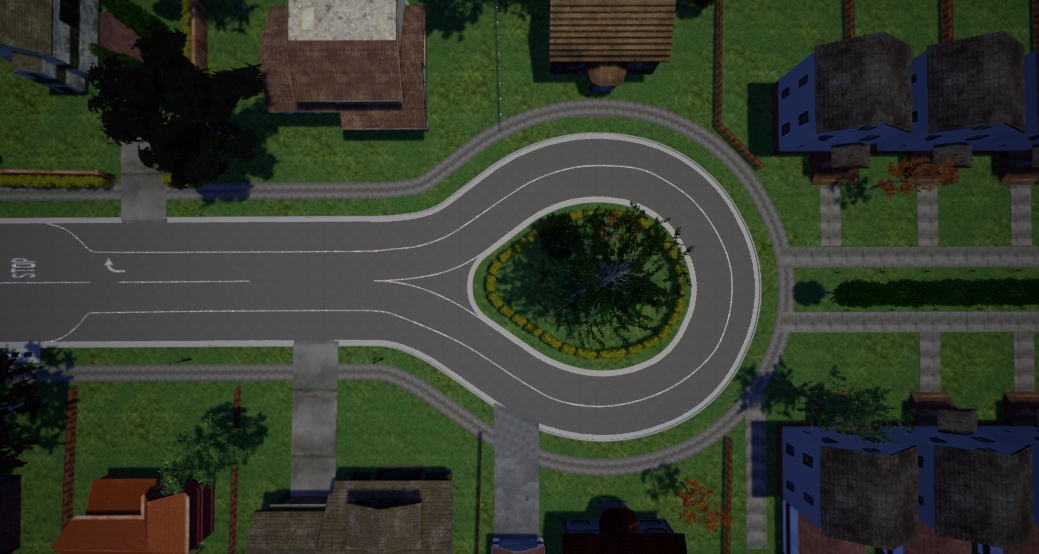
\includegraphics[width=.7\linewidth]{images/bundaran_tanpa_simpang}
	\caption{Bundaran Tanpa Simpang}
	\label{fig:bundaran_tanpa_simpang}
\end{figure}

\section{Sensor}
\label{sec:sensor}
Sensor menggunakan sensor kamera yang diletakkan secara fisik di bagian depan bawah dari agen. Sensor kamera yang digunakan adalah sensor kamera segmentasi. Sensor kamera segmentasi adalah sensor kamera yang memisahkan object-object di simulator menjadi berbagai warna unik yang solid. Citra yang dihasilkan dari sensor kamera segmentasi pada Gambar \ref{fig:segmentasi} adalah citra lanjutan yang telah di proses dari citra RGB pada gambar \ref{fig:citra_rgb}


\section{Akuisisi Data}
\label{sec:akuisisi_data}
Data citra diambil dari sensor dengan ukuran 480x270. Citra yang digunakan adalah citra segmentasi yang telah disediakan oleh sensor kamera segmentasi dari CARLA Simulator. Terlihat pada Gambar \ref{fig:citra_rgb} merupakan citra awal. Kemudian dilakukan segmentasi pada citra tersebut sehingga setiap obyek dipresentasikan dengan warna solid seperti pada Gambar \ref{fig:segmentasi}

\begin{figure}[H] 
	\centering
	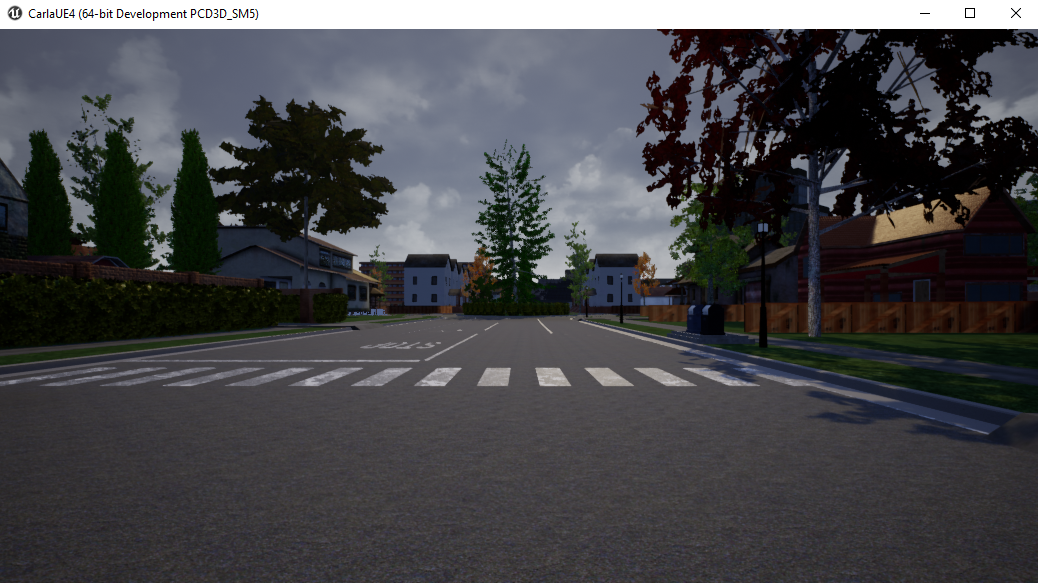
\includegraphics[width=.7\linewidth]{images/rgb}
	\caption{Citra RGB}
	\label{fig:citra_rgb}
\end{figure}
\begin{figure}[H] 
	\centering
	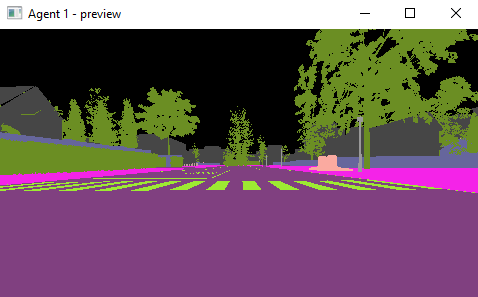
\includegraphics[width=.7\linewidth]{images/segmentasi}
	\caption{Citra Segmentasi}
	\label{fig:segmentasi}
\end{figure}
Ada dua jenis citra yang digunakan dalam tugas akhir ini, yaitu citra segmentasi grayscale dan citra segmentasi lanjutan.

Citra segmentasi grayscale merupakan citra segmentasi yang kemudian diberi filter grayscale agar dapat meminimalkan data yang dianalisa namun tetap mempertahankan fitur yang ada.

\begin{figure}[H] 
	\centering
	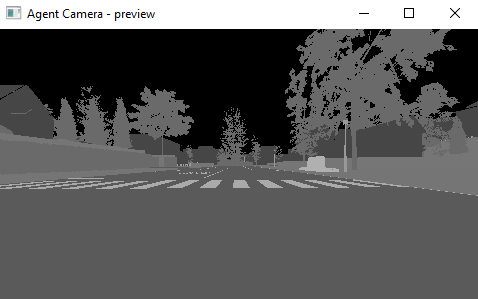
\includegraphics[width=.7\linewidth]{images/grayscale}
	\caption{Citra Segmentasi Grayscale}
	\label{fig:grayscale}
\end{figure}

Citra segmentasi lanjutan merupakan citra segmentasi, yang kemudian di segmentasi kembali menjadi dua jenis obyek, yaitu \textit{drivable }dan \textit{non-drivable}. Obyek \textit{drivable} dipresentasikan dengan warna putih dan obyek \textit{non-drivable} dipresentasikan dengan warna hitam.

\begin{figure}[H] 
	\centering
	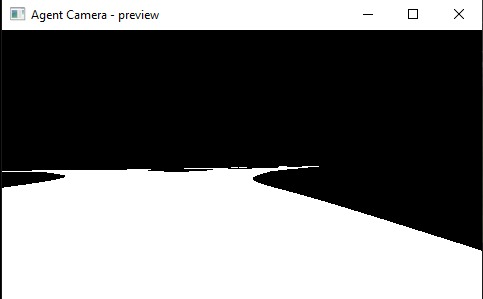
\includegraphics[width=.7\linewidth]{images/segmentasi_hitam_putih}
	\caption{Citra Segmentasi Lanjutan}
	\label{fig:segmentasi_hitam_putih}
\end{figure}

Citra segmentasi grayscale dan citra segmentasi lanjutan akan menjadi hasil akhir akuisi citra yang kemudian akan diberikan ke algoritma DQN untuk melakukan \textit{training} model dan/atau \textit{inference} model.

\section{\textit{Action}}
\label{sec:action}
Ada 3 \textit{action} yang bisa dilakukan oleh \textit{agent}. Diantaranya:

\begin{enumerate}[nolistsep]
	\item \verb=forward=
	
	\textit{Agent} \textit{throttle} dengan nilai 1 dan \textit{steer} dengan nilai 0. Dengan demikian agent akan melakukan gerakan manuver maju.
	
	\item \verb=forward_left=
	
	Agen \textit{throttle} dengan nilai 1 dan \textit{steer} dengan nilai -1. Dengan demikian agent akan melakukan gerakan manuver maju ke depan kiri.

	\item \verb=forward_right=
	
	Agen \textit{throttle} dengan nilai 1 dan \textit{steer} dengan nilai 1. Dengan demikian agent akan melakukan gerakan manuver maju ke depan kanan.
	
\end{enumerate}

\section{\textit{Reward Function}}
\label{sec:sistem_reward}

Fungsi reward dirancang agar mobil otonom mampu bergerak sepanjang lintasan dengan cepat dan aman.

\subsection{Bundaran Simpang Empat}Ada dua buah reward yang ditetapkan dimana masing-masing reward memperhatikan referensi \textit{target lane}. Target lane adalah garis imajiner yang menjadi target gerakan mobil otonom. Terlihat pada Gambar \ref{fig:target_lane_line}, \textit{target lane} digambarkan dengan titik-titik merah di sekitar bundaran.

\begin{figure}[H] 
	\centering
	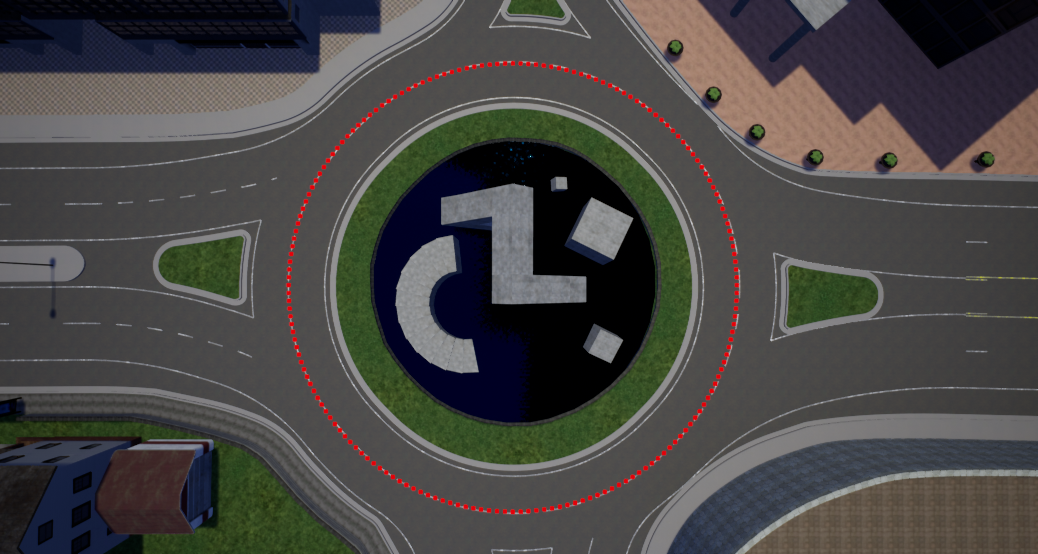
\includegraphics[width=1\linewidth]{images/target_lane_line}
	\caption{\textit{Target lane}}
	\label{fig:target_lane_line}
\end{figure}

\subsubsection{\textit{Reward} 1: Deviasi sudut dari \textit{target lane}}
Reward yang digunakan pada Reward 1 adalah 1/alpha. Alpha adalah sudut agent yang menyimpang dari \textit{target lane}. Teknis alpha dijelaskan pada Gambar \ref{fig:reward_anglediff_sketch}. 

\begin{figure}[H] 
	\centering
	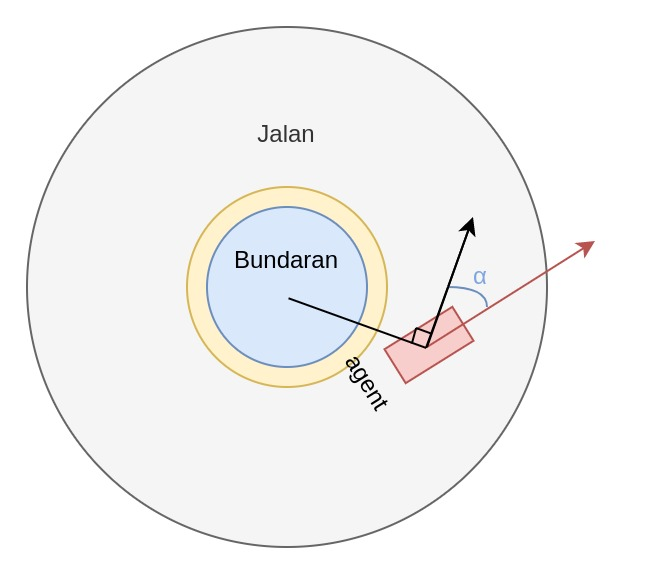
\includegraphics[width=1\linewidth]{images/reward_anglediff_sketch}
	\caption{Reward 1}
	\label{fig:reward_anglediff_sketch}
\end{figure}

Garis hitam merupakan vektor tegak lurus antara titik pusat bundaran ke titik pusat agen. Lalu garis merah adalah vektor arah mobil. Dari kedua nilai tersebut, didapat alpha yang merupakan sudut dari kedua vektor tersebut. Kemudian nilai reward didefinisikan dengan 1/alpha.

Potongan kode dari fungsi reward deviasi sudut terdapat pada Listing \ref{lst:reward_deviasi_sudut}.

\lstinputlisting[
language=Python,
caption={Reward Deviasi Sudut.},
label={lst:reward_deviasi_sudut}
]{program/reward_deviasi_sudut.py}

Terlihat pada potongan kode Listing \ref{lst:reward_deviasi_sudut} nilai tertinggi reward dibatasi menjadi 1. Hal ini dilakukan agar fluktuasi reward yang diberikan ke agent tidak terlalu tinggi untuk perubahan nilai yang kecil.


\subsubsection{\textit{Reward} 2: Deviasi jarak dari \textit{target lane}}
Reward yang digunakan pada reward 2 adalah \verb=1/deviasi_jarak*10=. Deviasi jarak adalah jarak terkecil agen terhadap \textit{target lane} dalam meter.

\begin{figure}[H] 
	\centering
	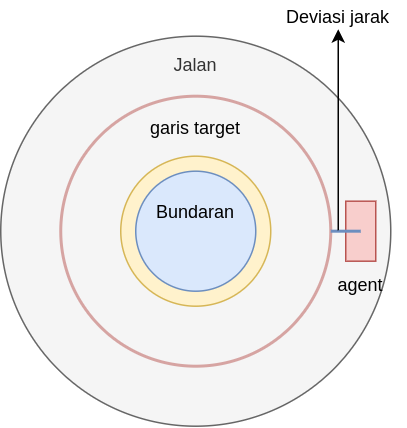
\includegraphics[width=.85\linewidth]{images/reward_deviasi_jarak}
	\caption{Reward 2}
	\label{fig:reward_deviasi_jarak}
\end{figure}

Potongan kode dari fungsi reward deviasi jarak terdapat pada Listing \ref{lst:reward_deviasi_jarak}.

\lstinputlisting[
language=Python,
caption={Reward Deviasi Jarak.},
label={lst:reward_deviasi_jarak}
]{program/reward_deviasi_jarak.py}

Terlihat pula pada potongan kode Listing \ref{lst:reward_deviasi_jarak} nilai tertinggi reward dibatasi menjadi 1. Hal ini dilakukan agar fluktuasi reward yang diberikan ke agent juga tidak terlalu tinggi untuk perubahan nilai yang kecil, seperti pada Reward 1.


Selain reward yang bernilai positif, diperlukan juga reward yang bernilai negatif untuk mengurangi peluang agent melakukan hal yang sebaiknya tidak dilakukan. Ada dua buah reward bernilai negatif yang diberikan.

\subsubsection{\textit{Reward} 3: Sentuhan dengan obyek lain}
Reward senilai -1 akan diberikan pada \textit{agent} jika agent menyentuh obyek lain selain jalan raya, tanah, dan trotoar.

Potongan kode dari fungsi reward sentuhan dengan obyek lain terdapat pada Listing \ref{lst:reward_car_collided}.

\lstinputlisting[
language=Python,
caption={Reward Sentuhan dengan Obyek Lain.},
label={lst:reward_car_collided}
]{program/reward_car_collided.py}

\subsubsection{\textit{Reward} 4: Deviasi jarak terlalu besar}
Reward senilai -0.5 akan diberikan pada \textit{agent} jika jarak antara \textit{agent} dan bundaran lebih besar dari 30 meter. Jarak 30 meter dari bundaran dapat dilihat di Gambar \ref{fig:punishment_lane_line}

\begin{figure}[H] 
	\centering
	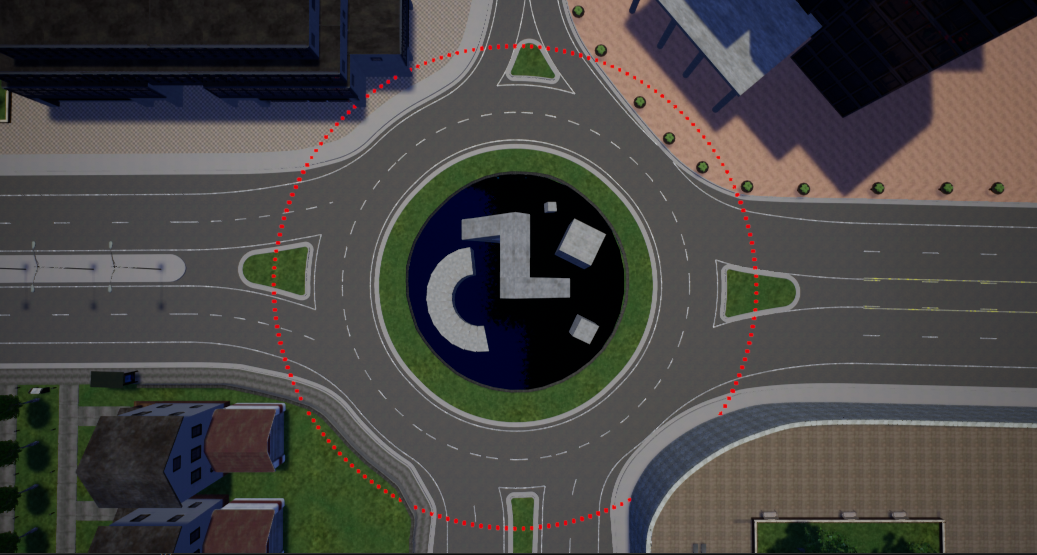
\includegraphics[width=1\linewidth]{images/punishment_lane_line}
	\caption{Batasan jarak}
	\label{fig:punishment_lane_line}
\end{figure}

Potongan kode dari fungsi reward deviasi jarak terlalu besar terdapat pada Listing \ref{lst:reward_too_far}.

\lstinputlisting[
language=Python,
caption={Reward Deviasi Jarak Terlalu Besar.},
label={lst:reward_too_far}
]{program/reward_too_far.py}


\subsubsection{\textit{Reward }Total}
Total nilai reward didefinisikan dengan Reward 1 + Reward 2 + Reward 3 + Reward 4.

\subsection{Bundaran Tanpa Simpang}
Pada bundaran tanpa simpang, fungsi reward yang diberikan berbeda. Pada kasus ini disediakan titik-titik jalur sebagai \textit{waypoint} yang harus diikuti oleh \textit{agent}.

\begin{figure}[H] 
	\centering
	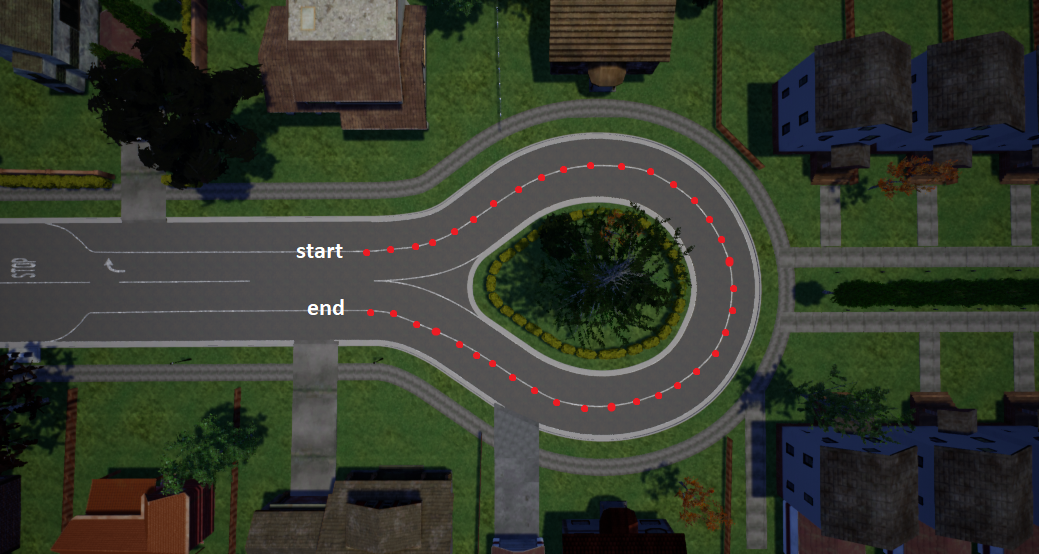
\includegraphics[width=1\linewidth]{images/waypoint}
	\caption{\textit{Waypoint}}
	\label{fig:waypoint}
\end{figure}

\textit{Waypoint} merupakan titik-titik pada map sebagai target tujuan jalannya \textit{agent}. Terlihat pada Gambar \ref{fig:waypoint}, titik-titik merah merupakan ilustrasi dari waypoint. Waypoint berjumlah 100 titik dimana setiap titiknya berjarak satu meter.

\subsubsection{\textit{Reward} Total}
Reward didefinisikan dengan 1/alpha. Alpha merupakan deviasi sudut arah \textit{agent }terhadap arah titik \textit{waypoint} terdekat dari \textit{agent} + 5.

\begin{figure}[H] 
	\centering
	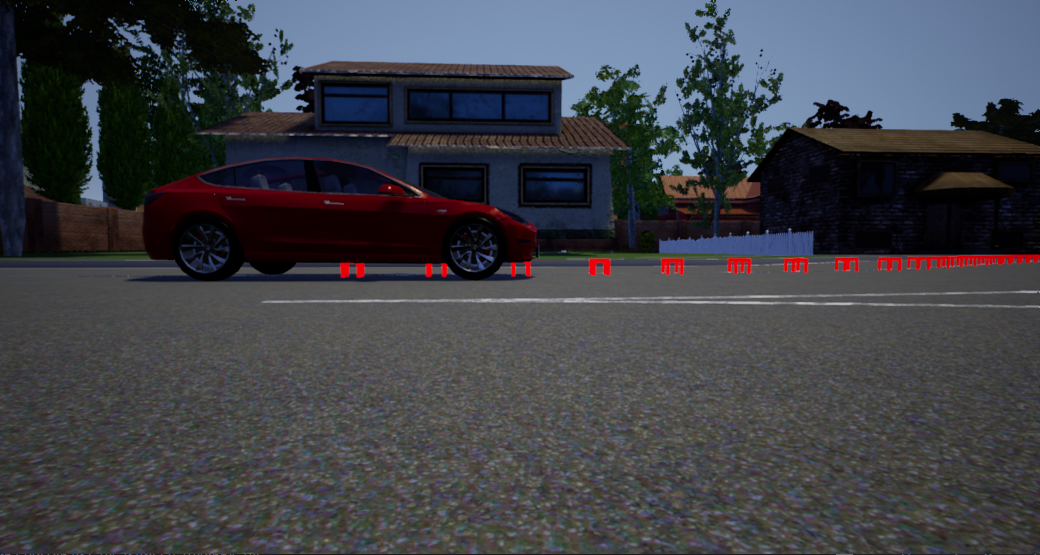
\includegraphics[width=1\linewidth]{images/waypoint_fromside}
	\caption{\textit{Waypoint }dari Sisi \textit{Agent}}
	\label{fig:waypoint_fromside}
\end{figure}

Gambar \ref{fig:waypoint_fromside} menunjukkan bahwa \textit{waypoint} terdekat + 5 dari \textit{agent} berjarak enam meter dari pusat koordinat \textit{agent}.

\begin{figure}[H] 
	\centering
	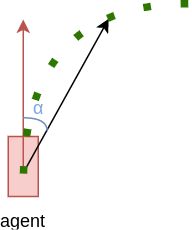
\includegraphics[width=.5\linewidth]{images/reward_alpha}
	\caption{Reward Alpha}
	\label{fig:reward_alpha}
\end{figure}

Ilustrasi fungsi reward dapat dilihat pada Gambar \ref{fig:reward_alpha}, dimana titik-titik hijau adalah \textit{waypoints}, garis merah adalah arah dari \textit{agent}, garis hitam adalah arah dari \textit{agent} ke \textit{waypoint}+5 dari \textit{agent}, serta alpha adalah perbedaan sudut dari kedua nilai sudut tersebut.

Potongan kode dari fungsi reward terdapat pada Listing \ref{lst:reward_alpha}.

\lstinputlisting[
language=Python,
caption={Reward Alpha.},
label={lst:reward_alpha}
]{program/reward_alpha.py}

Terlihat pula pada potongan kode Listing \ref{lst:reward_alpha} nilai tertinggi reward dibatasi menjadi 1. Hal ini dilakukan agar fluktuasi reward yang diberikan ke agent juga tidak terlalu tinggi untuk perubahan nilai yang kecil, seperti pada Reward 1 dan Reward 2 pada bundaran simpang empat.


\subsection{End Episode}
\label{sec:end_episode}
Waktu maksimal yang diberikan pada agent untuk melakukan proses learning setiap episodenya adalah 10 detik.

Episode akan berakhir jika waktu maksimal episode berakhir atau agent menyentuh object lain selain jalan raya, tanah, dan trotoar.

\section{Parameter DQN}
\label{sec:parameter_dqn}
Penentuan nilai hyperparameter yang tepat merupakan salah satu langkah yang penting dilakukan untuk mendapatkan model pembelajaran mesin yang baik. Dalam machine learning, hyperparameter adalah parameter yang digunakan untuk mengatur jalannya proses pembelajaran mesin. Berbeda dengan parameter model yang nilainya mengalami perubahan seiring berjalannya pembelajaran mesin, hyperparameter perlu didefinisikan di awal dan umumnya bernilai tetap sepanjang proses pembelajaran. Dalam tugas akhir ini, hyperparameter dari algoritma DQN didefinisikan sebagai berikut:

\subsection{Model}
\label{sec:model}
\begin{table}[H]
	\resizebox{\textwidth}{!}{%
		\begin{tabular}{|l|l|l|}
			\hline
			\textbf{Hyperparameter}   & \textbf{Nilai} & \textbf{Deskripsi}                                                                                                                            \\ \hline
			MINIBATCH\_SIZE           & 16             & \begin{tabular}[c]{@{}l@{}}Jumlah sampel pembelajaran yang\\ diproses oleh perhitungan SGD\\ (stochastic gradient) algoritma DQN\end{tabular} \\ \hline
			PREDICTION\_BATCH\_SIZE   & 1              & \begin{tabular}[c]{@{}l@{}}Jumlah sampel yang di prediksi\\ di saat yang bersamaan\end{tabular}                                               \\ \hline
			TRAINING\_BATCH\_SIZE     & 8              & \begin{tabular}[c]{@{}l@{}}Jumlah sampel yang di fit di saat\\ yang bersamaan (lebih besar lebih\\ cepat)\end{tabular}                        \\ \hline
			TRAINER\_MEMORY\_FRACTION & 0.6            &                                                                                                                                               \\ \hline
		\end{tabular}%
	}
\caption{Hyperparameter model.}
\label{tb:hyperparameter_model}
\end{table}

\iffalse
\begin{verbatim}
MINIBATCH_SIZE = 16
PREDICTION_BATCH_SIZE = 1
TRAINING_BATCH_SIZE = MINIBATCH_SIZE // 2
UPDATE_TARGET_EVERY = 100
TRAINER_MEMORY_FRACTION = 0.6
SAVE_CHECKPOINT_EVERY = 50
\end{verbatim}
\fi

\subsection{DQN}
\label{sec:dqn}

\begin{table}[H]
	\resizebox{\textwidth}{!}{%
		\begin{tabular}{|l|l|l|}
			\hline
			\textbf{Hyperparameter}   & \textbf{Nilai} & \textbf{Deskripsi}                                                                                                                            \\ \hline
			DISCOUNT                  & 0.99           & \begin{tabular}[c]{@{}l@{}}Nilai faktor discount dalam\\ perhitungan reward algoritma DQN\end{tabular}                                        \\ \hline
			REPLAY\_MEMORY\_SIZE      & 20\_000        & \begin{tabular}[c]{@{}l@{}}Berapa banyak step terakhir yang\\ disimpan untuk training model\end{tabular}                                      \\ \hline
			MIN\_REPLAY\_MEMORY\_SIZE & 5\_000         & \begin{tabular}[c]{@{}l@{}}Jumlah step minimum dalam\\ memori untuk memulai training\end{tabular}                                             \\ \hline
			OPTIMIZER\_LEARNING\_RATE & 0.001          & \begin{tabular}[c]{@{}l@{}}Laju pembelajaran yang digunakan\\ pada optimizer\end{tabular}                                                     \\ \hline
			OPTIMIZER\_DECAY          & 0.0            & \begin{tabular}[c]{@{}l@{}}Pengurangan laju pembelajaran\\ pada optimizer setiap episodenya\end{tabular}                                      \\ \hline
		\end{tabular}%
	}
	\caption{Hyperparameter DQN.}
	\label{tb:hyperparameter_dqn}
\end{table}

\iffalse
\begin{verbatim}
DISCOUNT = 0.99
REPLAY_MEMORY_SIZE = 20_000
MIN_REPLAY_MEMORY_SIZE = 5_000
\end{verbatim}
\fi

\subsection{Epsilon}

\begin{table}[H]
	\resizebox{\textwidth}{!}{%
		\begin{tabular}{|l|l|l|}
			\hline
			\textbf{Hyperparameter}   & \textbf{Nilai} & \textbf{Deskripsi}                                                                                                                            \\ \hline

			START\_EPSILON            & 1              & \begin{tabular}[c]{@{}l@{}}Nilai epsilon saat pertamakali\\ mulai training\end{tabular}                                                       \\ \hline
			EPSILON\_DECAY            & 0.9995         & \begin{tabular}[c]{@{}l@{}}Penurunan nilai epsilon di setiap\\ episodenya\end{tabular}                                                        \\ \hline
			MIN\_EPSILON              & 0.1            & \begin{tabular}[c]{@{}l@{}}Epsilon terendah yang\\ diperbolehkan\end{tabular}                                                                 \\ \hline
		\end{tabular}%
	}
	\caption{Hyperparameter epsilon.}
	\label{tb:hyperparameter_epsilon}
\end{table}
Penentuan parameter epsilon ditentukan oleh kondisi berikut. Epsilon akan bernilai 1 saat pertamakali memulai learning atau pada saat episode 0. Setiap dimulainya episode baru, nilai epsilon akan dikali dengan nilai 0.9995 hingga pada akhirnya akan bernilai 0.1 setelah 4700 episode. Pengurangan nilai epsilon akan berhenti setelah sampai pada nilai 0.1.

Penentuan parameter \textit{epsilon-greedy} ini dilakukan agar agent mampu melakukan kegiatan eksplorasi dan eksploitasi dengan tepat. Sehingga hasil yang didapatkan akan baik dalam waktu cepat.
\label{sec:epsilon}

\iffalse
\begin{verbatim}
START_EPSILON = 1
EPSILON_DECAY = 0.9995
MIN_EPSILON = 0.1
\end{verbatim}
\fi

\section{Arsitektur Model}
\label{sec:arsitektur_model}

Berikut adalah arsitektur yang digunakan:

\begin{table}[H]
	\begin{tabular}{lll}
		\textbf{Layer (type)}                      & \textbf{Output Shape}         & \textbf{Param \#} \\
		conv2d\_1\_input (InputLayer)     & (None, 270, 480, 1)  & 0        \\
		conv2d\_1 (Conv2D)                & (None, 270, 480, 64) & 640      \\
		activation\_1 (Activation)        & (None, 270, 480, 64) & 0        \\
		average\_pooling2d\_1 (AveragePoo & (None, 90, 160, 64)  & 0        \\
		conv2d\_2 (Conv2D)                & (None, 90, 160, 64)  & 36928    \\
		activation\_2 (Activation)        & (None, 90, 160, 64)  & 0        \\
		average\_pooling2d\_2 (AveragePoo & (None, 30, 54, 64)   & 0        \\
		conv2d\_3 (Conv2D)                & (None, 30, 54, 64)   & 36928    \\
		activation\_3 (Activation)        & (None, 30, 54, 64)   & 0        \\
		average\_pooling2d\_3 (AveragePoo & (None, 10, 18, 64)   & 0        \\
		flatten\_1 (Flatten)              & (None, 11520)        & 0        \\
		kmh\_input (InputLayer)           & (None, 1)            & 0        \\
		concatenate\_1 (Concatenate)      & (None, 11521)        & 0        \\
		dense\_1 (Dense)                  & (None, 256)          & 2949632  \\
		dense\_2 (Dense)                  & (None, 3)            & 771     
	\end{tabular}
\caption{Arsitektur model.}
\label{tb:arsitektur_model}
\end{table}

Diberikan konvolusi kepada citra image sebanyak 3 kali. Setiap konvolusi dilakukan dengan average pooling. Proses selanjutnya setelah konvolusi adalah menambahkan data kecepatan agent. Kemudian pada akhir dari proses akan didapatkan output action berjumlah 3.

Berikut adalah potongan program untuk model 64x3.
\lstinputlisting[
language=Python,
caption={Model 64x3.},
label={lst:bilanganprima}
]{program/model64x3.py}

Berikut adalah potongan program untuk hidden dense.
\lstinputlisting[
language=Python,
caption={Hidden dense.},
label={lst:bilanganprima}
]{program/hidden_dense.py}


\section{Training}
\label{sec:training}

\begin{figure}[H] 
	\centering
	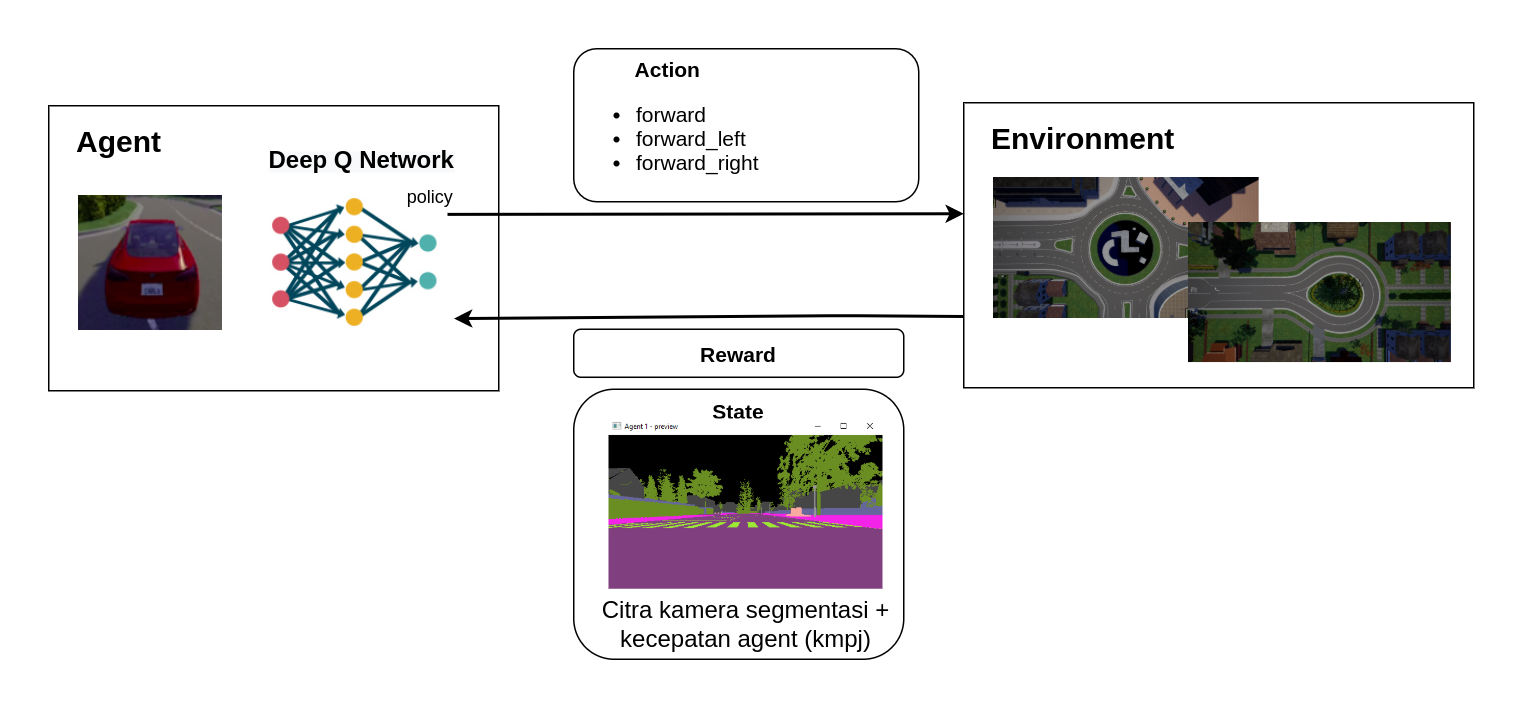
\includegraphics[width=1\linewidth]{images/metodologi}
	\caption{Diagram Blok Metodologi}
	\label{fig:blockdiagram}
\end{figure}

Proses training dilakukan setelah seluruh konfigurasi selesai dilakukan. Metodologi training dari tugas akhir ini terdapat pada Gambar \ref{fig:blockdiagram}. \textit{Agent} yang berada pada simulasi melakukan suatu \textit{action} yang menyebabkan berubahnya \textit{state}. \textit{State} yang berupa citra segmentasi dan kecepatan agent (kmpj) serta \textit{reward }dari \textit{agent} kemudian dikirimkan ke DQN untuk dilakukan training. Hasil dari training berupa \textit{policy },  akan menentukan\textit{action} yang kemudian akan dilaksanakan oleh \textit{agent}. Kemudian proses tersebut akan terulang kembali menjadi sebuah siklus yang tak henti.

\iffalse
Tugas akhir ini akan menggunakan metode \textit{deep reinforcement learning}, yaitu \textit{reinforcement learning }yang disertai dengan \textit{deep learning }untuk mempelajari \textit{policy }apa yang cocok untuk digunakan oleh \textit{agent}. 

Algoritma deep reinforcement learning yang digunakan adalah Deep Q Network (DQN). Deep Q Network merupakan implementasi neural network atau deep learning pada Q-learning.

Parameter yang diberikan pada DQN adalah citra yang telah di segmentasi lalu diubah menjadi grayscale, serta kecepatan kendaraan dalam nilai kmpj.
\fi





%-----------------------------
%END for C and Python template
\iffalse
% Contoh pembuatan potongan kode
\begin{lstlisting}[
  language=C++,
  caption={Program halo dunia.},
  label={lst:halodunia}
]
#include <iostream>

int main() {
    std::cout << "Halo Dunia!";
    return 0;
}
\end{lstlisting}

% Contoh input potongan kode dari file
\lstinputlisting[
  language=Python,
  caption={Program perhitungan bilangan prima.},
  label={lst:bilanganprima}
]{program/bilangan-prima.py}

\lipsum[4]
\fi
